\documentclass[]{article}
\usepackage{lmodern}
\usepackage{amssymb,amsmath}
\usepackage{ifxetex,ifluatex}
\usepackage{fixltx2e} % provides \textsubscript
\ifnum 0\ifxetex 1\fi\ifluatex 1\fi=0 % if pdftex
  \usepackage[T1]{fontenc}
  \usepackage[utf8]{inputenc}
\else % if luatex or xelatex
  \ifxetex
    \usepackage{mathspec}
  \else
    \usepackage{fontspec}
  \fi
  \defaultfontfeatures{Ligatures=TeX,Scale=MatchLowercase}
\fi
% use upquote if available, for straight quotes in verbatim environments
\IfFileExists{upquote.sty}{\usepackage{upquote}}{}
% use microtype if available
\IfFileExists{microtype.sty}{%
\usepackage{microtype}
\UseMicrotypeSet[protrusion]{basicmath} % disable protrusion for tt fonts
}{}
\usepackage[margin=1in]{geometry}
\usepackage{hyperref}
\hypersetup{unicode=true,
            pdftitle={Principal Component Analysis},
            pdfauthor={Dataset new\_data},
            pdfborder={0 0 0},
            breaklinks=true}
\urlstyle{same}  % don't use monospace font for urls
\usepackage{color}
\usepackage{fancyvrb}
\newcommand{\VerbBar}{|}
\newcommand{\VERB}{\Verb[commandchars=\\\{\}]}
\DefineVerbatimEnvironment{Highlighting}{Verbatim}{commandchars=\\\{\}}
% Add ',fontsize=\small' for more characters per line
\usepackage{framed}
\definecolor{shadecolor}{RGB}{248,248,248}
\newenvironment{Shaded}{\begin{snugshade}}{\end{snugshade}}
\newcommand{\KeywordTok}[1]{\textcolor[rgb]{0.13,0.29,0.53}{\textbf{#1}}}
\newcommand{\DataTypeTok}[1]{\textcolor[rgb]{0.13,0.29,0.53}{#1}}
\newcommand{\DecValTok}[1]{\textcolor[rgb]{0.00,0.00,0.81}{#1}}
\newcommand{\BaseNTok}[1]{\textcolor[rgb]{0.00,0.00,0.81}{#1}}
\newcommand{\FloatTok}[1]{\textcolor[rgb]{0.00,0.00,0.81}{#1}}
\newcommand{\ConstantTok}[1]{\textcolor[rgb]{0.00,0.00,0.00}{#1}}
\newcommand{\CharTok}[1]{\textcolor[rgb]{0.31,0.60,0.02}{#1}}
\newcommand{\SpecialCharTok}[1]{\textcolor[rgb]{0.00,0.00,0.00}{#1}}
\newcommand{\StringTok}[1]{\textcolor[rgb]{0.31,0.60,0.02}{#1}}
\newcommand{\VerbatimStringTok}[1]{\textcolor[rgb]{0.31,0.60,0.02}{#1}}
\newcommand{\SpecialStringTok}[1]{\textcolor[rgb]{0.31,0.60,0.02}{#1}}
\newcommand{\ImportTok}[1]{#1}
\newcommand{\CommentTok}[1]{\textcolor[rgb]{0.56,0.35,0.01}{\textit{#1}}}
\newcommand{\DocumentationTok}[1]{\textcolor[rgb]{0.56,0.35,0.01}{\textbf{\textit{#1}}}}
\newcommand{\AnnotationTok}[1]{\textcolor[rgb]{0.56,0.35,0.01}{\textbf{\textit{#1}}}}
\newcommand{\CommentVarTok}[1]{\textcolor[rgb]{0.56,0.35,0.01}{\textbf{\textit{#1}}}}
\newcommand{\OtherTok}[1]{\textcolor[rgb]{0.56,0.35,0.01}{#1}}
\newcommand{\FunctionTok}[1]{\textcolor[rgb]{0.00,0.00,0.00}{#1}}
\newcommand{\VariableTok}[1]{\textcolor[rgb]{0.00,0.00,0.00}{#1}}
\newcommand{\ControlFlowTok}[1]{\textcolor[rgb]{0.13,0.29,0.53}{\textbf{#1}}}
\newcommand{\OperatorTok}[1]{\textcolor[rgb]{0.81,0.36,0.00}{\textbf{#1}}}
\newcommand{\BuiltInTok}[1]{#1}
\newcommand{\ExtensionTok}[1]{#1}
\newcommand{\PreprocessorTok}[1]{\textcolor[rgb]{0.56,0.35,0.01}{\textit{#1}}}
\newcommand{\AttributeTok}[1]{\textcolor[rgb]{0.77,0.63,0.00}{#1}}
\newcommand{\RegionMarkerTok}[1]{#1}
\newcommand{\InformationTok}[1]{\textcolor[rgb]{0.56,0.35,0.01}{\textbf{\textit{#1}}}}
\newcommand{\WarningTok}[1]{\textcolor[rgb]{0.56,0.35,0.01}{\textbf{\textit{#1}}}}
\newcommand{\AlertTok}[1]{\textcolor[rgb]{0.94,0.16,0.16}{#1}}
\newcommand{\ErrorTok}[1]{\textcolor[rgb]{0.64,0.00,0.00}{\textbf{#1}}}
\newcommand{\NormalTok}[1]{#1}
\usepackage{graphicx,grffile}
\makeatletter
\def\maxwidth{\ifdim\Gin@nat@width>\linewidth\linewidth\else\Gin@nat@width\fi}
\def\maxheight{\ifdim\Gin@nat@height>\textheight\textheight\else\Gin@nat@height\fi}
\makeatother
% Scale images if necessary, so that they will not overflow the page
% margins by default, and it is still possible to overwrite the defaults
% using explicit options in \includegraphics[width, height, ...]{}
\setkeys{Gin}{width=\maxwidth,height=\maxheight,keepaspectratio}
\IfFileExists{parskip.sty}{%
\usepackage{parskip}
}{% else
\setlength{\parindent}{0pt}
\setlength{\parskip}{6pt plus 2pt minus 1pt}
}
\setlength{\emergencystretch}{3em}  % prevent overfull lines
\providecommand{\tightlist}{%
  \setlength{\itemsep}{0pt}\setlength{\parskip}{0pt}}
\setcounter{secnumdepth}{0}
% Redefines (sub)paragraphs to behave more like sections
\ifx\paragraph\undefined\else
\let\oldparagraph\paragraph
\renewcommand{\paragraph}[1]{\oldparagraph{#1}\mbox{}}
\fi
\ifx\subparagraph\undefined\else
\let\oldsubparagraph\subparagraph
\renewcommand{\subparagraph}[1]{\oldsubparagraph{#1}\mbox{}}
\fi

%%% Use protect on footnotes to avoid problems with footnotes in titles
\let\rmarkdownfootnote\footnote%
\def\footnote{\protect\rmarkdownfootnote}

%%% Change title format to be more compact
\usepackage{titling}

% Create subtitle command for use in maketitle
\newcommand{\subtitle}[1]{
  \posttitle{
    \begin{center}\large#1\end{center}
    }
}

\setlength{\droptitle}{-2em}

  \title{Principal Component Analysis}
    \pretitle{\vspace{\droptitle}\centering\huge}
  \posttitle{\par}
    \author{Dataset new\_data}
    \preauthor{\centering\large\emph}
  \postauthor{\par}
    \date{}
    \predate{}\postdate{}
  

\begin{document}
\maketitle

This dataset contains 150 individuals and 2 variables.

\begin{center}\rule{0.5\linewidth}{\linethickness}\end{center}

\subsubsection{1. Study of the outliers}\label{study-of-the-outliers}

The analysis of the graphs does not detect any outlier.

\begin{center}\rule{0.5\linewidth}{\linethickness}\end{center}

\subsubsection{2. Inertia distribution}\label{inertia-distribution}

The inertia of the first dimensions shows if there are strong
relationships between variables and suggests the number of dimensions
that should be studied.

The first two dimensions of PCA express \textbf{100\%} of the total
dataset inertia ; that means that 100\% of the individuals (or
variables) cloud total variability is explained by the plane. The
inertia observed on the first plane is smaller than the reference value
that equals \textbf{100\%}, therefore low in comparison (the reference
value is the 0.95-quantile of the inertia percentages distribution
obtained by simulating 1429 data tables of equivalent size on the basis
of a normal distribution). However, the inertia related to the first
dimension is greater than the reference value \textbf{57.75\%}. Even if
the inertia projected on the first plane is not significant, these
explained by the first dimension is significant.

\begin{center}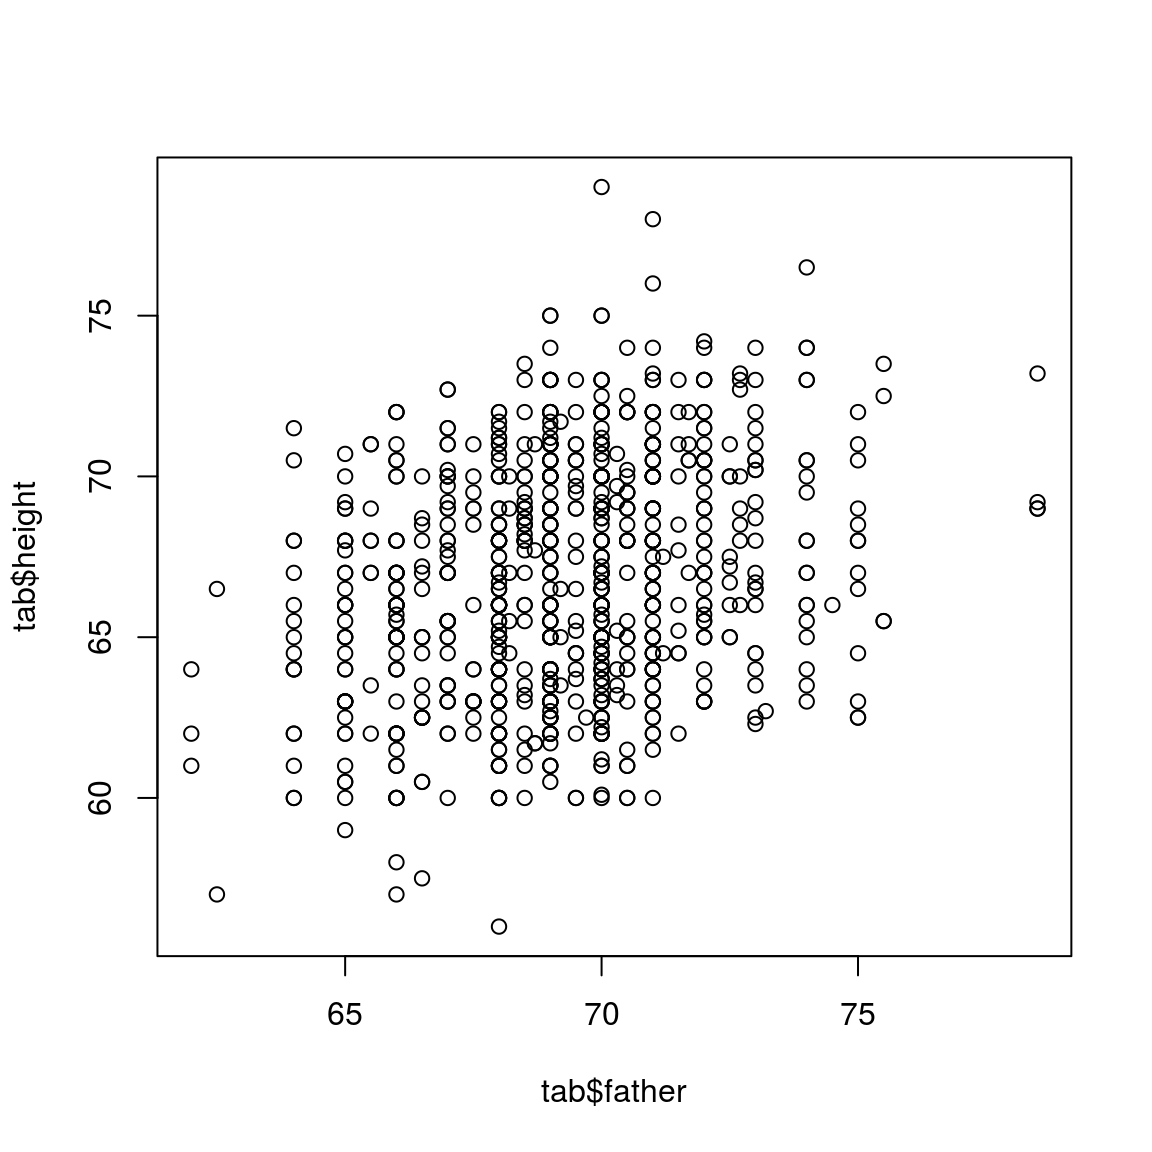
\includegraphics{Investigate_files/figure-latex/unnamed-chunk-3-1} \end{center}

\textbf{Figure 2 - Decomposition of the total inertia on the components
of the PCA} \emph{The first factor is largely dominant: it expresses
itself 98.14\% of the data variability.} \emph{Note that in such a case,
the variability related to the other components might be meaningless,
despite of a high percentage.}

An estimation of the right number of axis to interpret suggests to
restrict the analysis to the description of the first 1 axis. These axis
present an amount of inertia greater than those obtained by the
0.95-quantile of random distributions (98.14\% against 57.75\%). This
observation suggests that only this axis is carrying a real information.
As a consequence, the description will stand to these axis.

\begin{center}\rule{0.5\linewidth}{\linethickness}\end{center}

\subsubsection{3. Description of the dimension
1}\label{description-of-the-dimension-1}

\begin{center}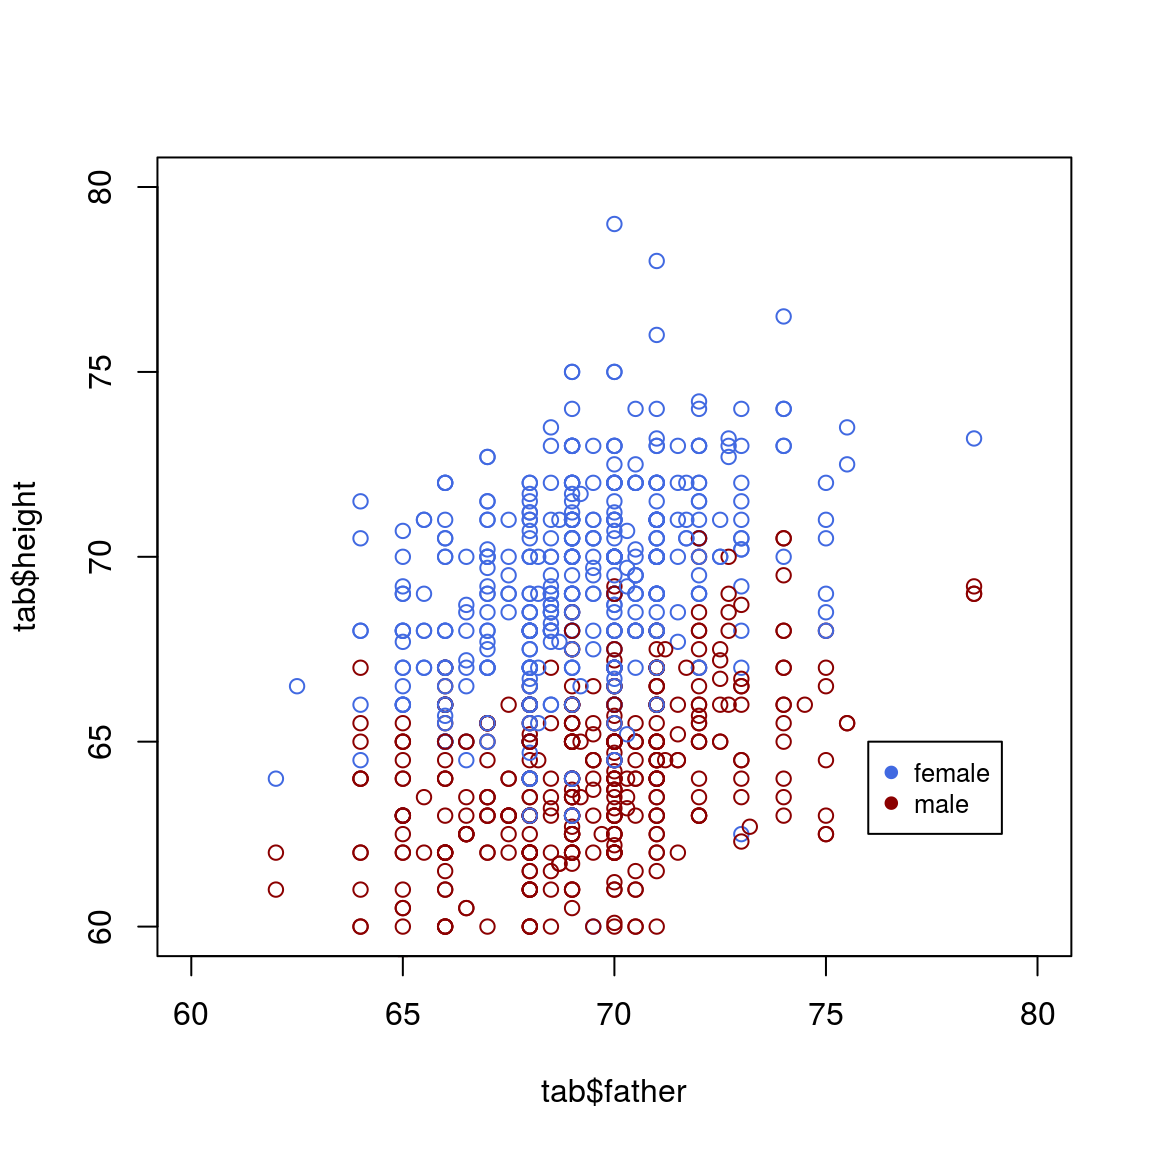
\includegraphics{Investigate_files/figure-latex/unnamed-chunk-4-1} \end{center}

\textbf{Figure 3.1 - Individuals factor map (PCA)} \emph{The labeled
individuals are those with the higher contribution to the plane
construction.}

\begin{center}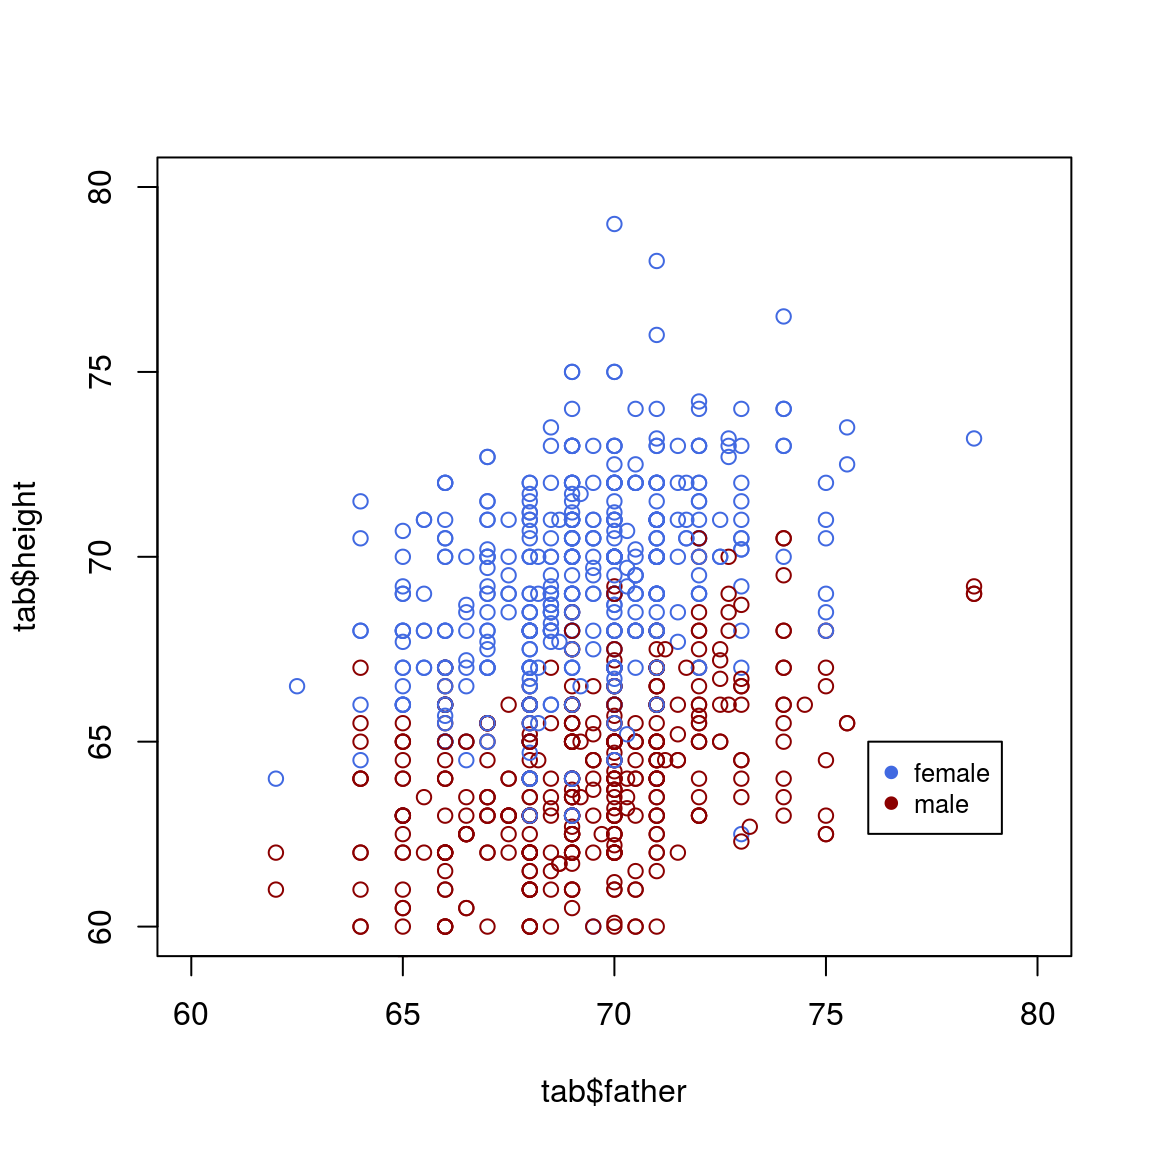
\includegraphics{Investigate_files/figure-latex/unnamed-chunk-5-1} \end{center}

\textbf{Figure 3.2 - Variables factor map (PCA)} \emph{The labeled
variables are those the best shown on the plane.}

\begin{center}\rule{0.5\linewidth}{\linethickness}\end{center}

The \textbf{dimension 1} opposes individuals such as \emph{108},
\emph{115}, \emph{116}, \emph{123}, \emph{130}, \emph{135} and
\emph{142} (to the right of the graph, characterized by a strongly
positive coordinate on the axis) to individuals characterized by a
strongly negative coordinate on the axis (to the left of the graph).

The group in which the individuals \emph{108}, \emph{115}, \emph{116},
\emph{123}, \emph{130}, \emph{135} and \emph{142} stand (characterized
by a positive coordinate on the axis) is sharing :

\begin{itemize}
\tightlist
\item
  high values for the variables \emph{petal\_width} and
  \emph{petal\_length} (variables are sorted from the strongest).
\end{itemize}

The group 2 (characterized by a negative coordinate on the axis) is
sharing :

\begin{itemize}
\tightlist
\item
  low values for the variables \emph{petal\_length} and
  \emph{petal\_width} (variables are sorted from the weakest).
\end{itemize}

Note that the variables \emph{petal\_length} and \emph{petal\_width} are
highly correlated with this dimension (respective correlation of 0.98,
0.98). These variables could therefore summarize themselve the dimension
1.

\begin{center}\rule{0.5\linewidth}{\linethickness}\end{center}

\subsubsection{4. Classification}\label{classification}

\begin{center}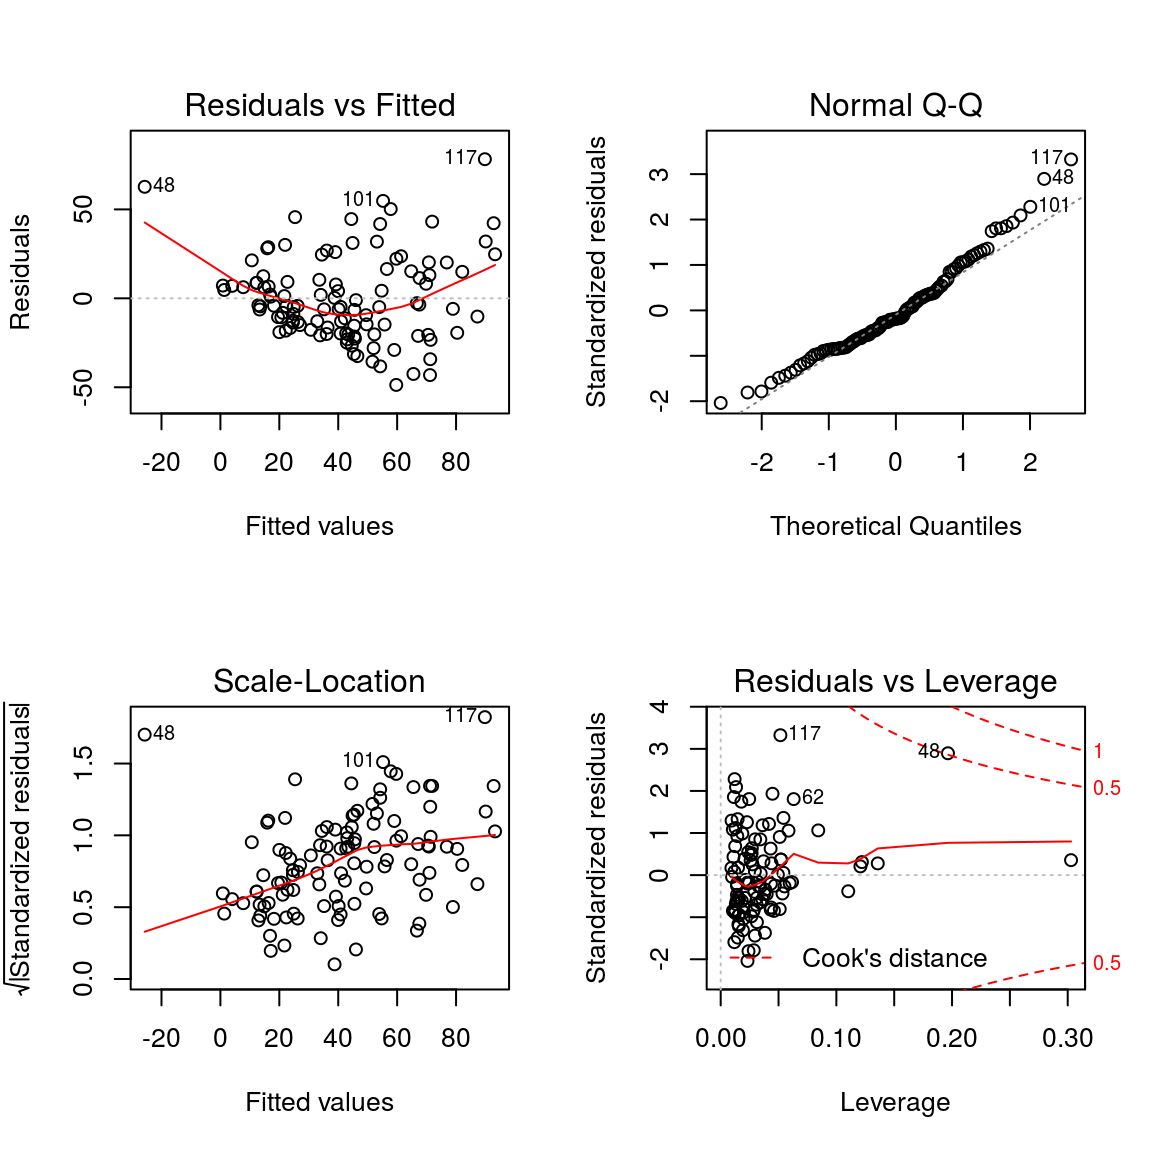
\includegraphics{Investigate_files/figure-latex/unnamed-chunk-7-1} \end{center}

\textbf{Figure 4 - Ascending Hierarchical Classification of the
individuals.} \emph{The classification made on individuals reveals 3
clusters.}

The \textbf{cluster 1} is made of individuals sharing :

\begin{itemize}
\tightlist
\item
  low values for the variables \emph{petal\_length} and
  \emph{petal\_width} (variables are sorted from the weakest).
\end{itemize}

The \textbf{cluster 2} is made of individuals such as \emph{135}. This
group is characterized by :

\begin{itemize}
\tightlist
\item
  high values for the variable \emph{petal\_length}.
\end{itemize}

The \textbf{cluster 3} is made of individuals such as \emph{108},
\emph{115}, \emph{116}, \emph{123}, \emph{130}, \emph{137}, \emph{142},
\emph{145} and \emph{146}. This group is characterized by :

\begin{itemize}
\tightlist
\item
  high values for the variables \emph{petal\_width} and
  \emph{petal\_length} (variables are sorted from the strongest).
\end{itemize}

\begin{center}\rule{0.5\linewidth}{\linethickness}\end{center}

\subsection{Annexes}\label{annexes}

\begin{Shaded}
\begin{Highlighting}[]
\KeywordTok{dimdesc}\NormalTok{(res, }\DataTypeTok{axes =} \DecValTok{1}\OperatorTok{:}\DecValTok{1}\NormalTok{)}
\end{Highlighting}
\end{Shaded}

\begin{verbatim}
$Dim.1
$Dim.1$quanti
             correlation       p.value
petal_width    0.9906455 6.325627e-130
petal_length   0.9906455 6.325627e-130
\end{verbatim}

\textbf{Figure 5 - List of variables characterizing the dimensions of
the analysis.}

\begin{Shaded}
\begin{Highlighting}[]
\NormalTok{res.hcpc}\OperatorTok{$}\NormalTok{desc.var}
\end{Highlighting}
\end{Shaded}

\begin{verbatim}

Link between the cluster variable and the quantitative variables
================================================================
                  Eta2      P-value
petal_width  0.9414745 2.511036e-91
petal_length 0.9382122 1.353088e-89

Description of each cluster by quantitative variables
=====================================================
$`1`
                v.test Mean in category Overall mean sd in category
petal_width  -10.83344            0.244     1.198667      0.1061320
petal_length -11.26285            1.464     3.758667      0.1717673
             Overall sd      p.value
petal_width   0.7606126 2.390051e-27
petal_length  1.7585292 2.001863e-29

$`2`
               v.test Mean in category Overall mean sd in category
petal_length 2.717692         4.296154     3.758667      0.5003697
             Overall sd     p.value
petal_length   1.758529 0.006573892

$`3`
               v.test Mean in category Overall mean sd in category
petal_width  9.441184         2.056250     1.198667      0.2397101
petal_length 8.609194         5.566667     3.758667      0.5432669
             Overall sd      p.value
petal_width   0.7606126 3.685897e-21
petal_length  1.7585292 7.357580e-18
\end{verbatim}

\textbf{Figure 6 - List of variables characterizing the clusters of the
classification.}


\end{document}
